% \begin{savequote}[8cm]
% Alles Gescheite ist schon gedacht worden.\\
% Man muss nur versuchen, es noch einmal zu denken.

% All intelligent thoughts have already been thought;\\
% what is necessary is only to try to think them again.
%   \qauthor{--- Johann Wolfgang von Goethe \cite{von_goethe_wilhelm_1829}}
% \end{savequote}

\chapter{\label{ch:xailimitations}Limitations of Post-Hoc Explainable AI}

\minitoc

\section{Introduction}
Increasingly, decisions affecting the lives of lay people are made by AI algorithms. And while these algorithms may be useful, they can also be dangerous. Users of AI systems desire an understanding of how these systems functions and why they yield the outputs they do, so that they may respond appropriately to the outputs \cite{binns_human_2022}. When AI systems make decisions impacting the user, user insight into the decision-making process allows for recourse \cite{ustun_actionable_2019}. However, when decision-making systems involve both an AI and human component, user insight into AI outputs is crucial in both (1) inducing appropriate reliance or scepticism in the AI as warranted and (2) optimising the overall performance of the decision-making system. This is especially true in high-stakes domains such as healthcare, finance, and criminal justice, where the decisions made by AI systems can have significant consequences for individuals \cite{binns_human_2022,ustun_actionable_2019,wachter_counterfactual_2017}.

The growing field of Explainable Artificial Intelligence (xAI) aims to develop methods for explaining algorithms. While some models are intrinsically interpretable \cite{rudin_interpretable_2021}, many more complicated machine learning algorithms are difficult to interpret. In order to explain these more complex models, various dedicated explanation algorithms have been proposed. Within the field of xAI, post-hoc, model-agnostic explainability methods remain popular due to their flexibility and ease-of-application \cite{molnar_interpretable_2019}. Indeed, the ability of methods like SHAP, LIME, and Scoped Anchors to treat any model as a black-box allows for applications of explainability to models that would be otherwise inscrutable \cite{lundberg_unified_2017,ribeiro_why_2016,ribeiro_anchors_2018}. However, there are several known limitations that can impact their utility as IAIDSTs; in some cases, these limitations undermine the purpose of explanation, or even to deceive and mislead users \cite{wang_transparency_2022}. 

In this Chapter, we explore a disconnect between user trust in an AI system and that system's trustworthiness as a result of post-hoc explainable AI tools. We begin by citing a series of papers yielding this result in a variety of contexts, and proceed to present our own work confirming that this disconnect persists in talent identification tasks. We then identify theories of when and why this disconnect occurs, and propose a series of experiments to test these theories. 

In Chapter \ref{ch:usingxai}, we implement these experiments and present the results.

\section{Trust and Trustworthiness in Explainable AI}
\emph{User trust is central to the utility and limitations of any user-facing system. In the context of IAIDSTs, user trust in the system facilitates the system's adoption and use. Explainability is crucial here, as an oft-cited goal of transparency is increasing user trust in AI systems. However, though trust is much-discussed, trustworthiness is often overlooked. Here, we examine literature pertaining to the relationship between trust and trustworthiness, especially in the context of explainable AI. We revisit the framework for trust posited in Chapter \ref{ch:background}, and discuss the limitations this places on trustworthy explainability systems.}

\textcite{jacovi_formalizing_2021} set out rules for trust in an algorithmic context. They set out a basic philosophical analysis of trust (in the general, non-algorithmic sense): A trusts B if and only if A believes that B will act in A's best interest and accepts vulnerability to B's actions. Trust often has limited scope; typically, A will trust B regarding some particular actions or motivations, but not others.

In the context of trust in AI, this definition is only slightly changed. \textcite{jacovi_formalizing_2021} characterise trust in an AI system by two properties: ``the vulnerability of the user, and the ability to anticipate the impact of the AI model's decisions''; \textcite{vereschak_how_2021} similarly isolate three elements: ``trust is linked to a situation of vulnerability and positive expectations, and is an attitude''; \textcite{lee_trust_2004} give a similar definition of trust: ``An attitude that an agent will achieve an individual's goal in a situation characterized by uncertainty and vulnerability''. In all definitions, we see \emph{vulnerability} emerge as a key concept, and we variably also see that trust is characterised by \emph{uncertainty} and \emph{expectations}.

An important distinction here can be drawn between whether someone or something is trusted and whether that trust is well-placed; i.e. it is worthy of trust \cite{hardin_trust_2002}. In the machine context, \textcite{jacovi_formalizing_2021} argue, an algorithm is worthy of trust if and only if there exists some contract that the algorithm promises (or that the algorithm's creators and implementors promise) to uphold. They term this a `contractual' model of trust. We adopt the nomenclature of contractual trust and use it to frame breakdowns in trust in specific post-hoc explanations.

\section{A Series of Concerning Results}
\emph{It is important that users be led to place appropriate, calibrated trust in the AI systems they rely on. Exploring the literature, we find that, in many cases, post-hoc explanations of AI outputs increase user trust in the AI system..}

\subsection{The Dangers of Transparency}
It is often assumed in the xAI literature that transparency of AI systems is always desirable \cite{molnar_interpretable_2019,miller_explanation_2017-1}. However, \textcite{wang_transparency_2022} dispel this claim. In particular, they demonstrate how, rather than empowering users and stakeholders, some implementations of algorithmic transparency serve the system's deployers, rather than its users, either through a false sense of understanding or the enforcement of norms and power structures. They examine the USA's FICO credit score, which releases the factors that go into the score, the data sources for these factors, and general guidelines on how these factors are used. They find specific information on the use of these factors lacking, and conclude that, rather than empowering users to debate the ethics of certain decisions, this transparency only serves to enforce certain behaviours among the users \cite{wang_transparency_2022}.

\textcite{ustun_actionable_2019} note a similar danger in transparency. They argue that explanations of AI systems making decisions about at end-users should empower those end users to alter the system's determinations. In particular, they introduce the concept of `Actionable Recourse', which consists of a specific set of actions an end-user can take to change the AI's determination, and demonstrate how to calculate these for linear models. Key to actionable recourse is that the actions an explainee should take in response to the explanation are clear in the explanation \cite{ustun_actionable_2019}.

We extend this concept to the context of IAIDSTs. Explanations aimed at decision-makers need not provide them \emph{recourse}, as decision-makers already posses the ability to override the AI system. However, they should still provide \emph{actionable} information, so that the explanations should contain information relevant to the decision-makers choice of what to do with the machine recommendation.

\subsection{Black Box Explanations Increase User Trust in AI Systems}
A number of studies exploring popular post-hoc, black-box explanation algorithms have found that these methods tend to increase overall user trust in the system being explained \cite{ford_play_2020,jacobs_how_2021,wang_transparency_2022}. 

\textcite{ford_play_2020} explore this effect in the context of a machine decision-maker with a human evaluator. They run a study examining the impact of post-hoc explanations-by-example and error-rates on people's perceptions of a black-box classifier classifying images from the MNIST dataset. They show that presenting `case-based explanations' (a series of three important data points in the training of the model; elsewhere, we term this an `influential instances' explanation and use `case-based' more broadly) lead participants to perceive miss-classifications as more correct \cite{ford_play_2020}.

\textcite{jacobs_how_2021} extend this result to a human-in-the-loop context. They study the effect of machine recommendation on a clinician's ability to select antidepressant treatments, and find that providing clinicians an incorrect algorithmically generated treatment list lowers the accuracy of clinicians' own treatment lists. Notably, they do not isolate this result to the presence of an explanation, but rather demonstrate how two explainable AI systems harm clinician antidepressant selection relative to a placebo group. However, they also find that feature-based explanations mislead clinicians more than heuristic-based explanations. Modern best practices outlined by \textcite{miller_explanation_2017-1} prefer the usage of feature-based explanations, so we find this particularly alarming \cite{jacobs_how_2021}.

\textcite{mccradden_when_2021} responds to \textcite{jacobs_how_2021} questioning the role of accuracy in explanations of IAIDSTs. They note the focus of \textcite{jacobs_how_2021} on improving \emph{accuracy} of the treatment lists, and aim to do this with IAIDSTs. However, though these systems may optimise for accuracy, they notably fail (at least in these specific instances) to facilitate clinicians' ability to \emph{help patients}, which is a clinicians' primary goal \cite{mccradden_when_2021}.

In a broader context, while `helping patients' doesn't describe the goal of all IAIDSTs, neither does `improving accuracy'. And, though increasing decision-maker trust regardless of system veracity may improve overall accuracy, it may hamper the broader goal of the decision-making system.

\subsection{Impacts on Talent Identification}
It should be noted that these effects are not universal. \textcite{mohseni_trust_nodate} measure user trust in an AI fake news detection system over time, and find the profile of the users to be just as important as the type of explanation. Though they demonstrate that different explanatory conditions have differential effects on which profile participants are likely to exhibit, they also cluster trust into five profiles by user: consistent over-trust, consistent under-trust, consistent trust, trust gains continually, and trust decreases continually. These profiles suggest that the same explanations will impact different groups performing different tasks differently. Thus, while an IAIDST may lead clinicians selecting antidepressants astray, it may have no effect (or even the opposite effect) on talent identification tasks \cite{mohseni_trust_nodate}.

In the next section, we undertake a series of experiments to test the implications of these limitations for talent identification.

\section{Misleading Explanations of AI Outputs in Talent Identification}
\emph{Explainable AI (xAI) methods are often motivated by the need to increase user trust in AI systems. However, as we have explored above, increased trust may not always be desirable. While unwarranted distrust might lead people to neglect AI systems when they are correct, unwarranted trust can also be a risk. Explanations which encourage unwarranted trust in incorrect AI outputs might mislead humans into making bad decisions. We investigate the extent to which three different xAI methods create too much trust in their underlying AI systems. Examining SHAP, Scoped Anchors, and a `Confidence' explanation that presents the model's confidence in an output, we conduct experiments where participants perform tasks with xAI assistance. We find that when the system is wrong, SHAP or Confidence explanations still increase trust. Scoped Anchors explanations, by contrast, increase participants' confidence in their own estimations regardless of the system's correctness. We discuss implications for the design and deployment of xAI in human-in-the-loop tasks.}

\subsection{The Studies}
We design two studies to answer the question: ``Can explanations of AI outputs create unwarranted user trust in those outputs?''. In particular, we restrict our research question to tasks familiar to lay people with a well-defined but difficult-to-ascertain ground truth. Furthermore, to help make comparisons to related works, we select tasks common in xAI research. Our two tasks are: \emph{estimating a hypothetical person's salary} based on census information of that individual, and \emph{predicting whether someone will be severely delinquent in making a credit payment}. We use two datasets: the Adult dataset collected in the 1994 US Census and curated by \textcite{kohavi_scaling_1996} and the Give Me Some Credit dataset curated by \textcite{GiveMeSomeCredit}. In both tasks, the participant aims to accurately estimate the dependent variable with the help of the AI system and one of several possible explanations of the AI system's estimate (which is possibly just the confidence rating of the model). More detail on the selection of our tasks can be found in Appendix \ref{app:misleadingexplanations}.

We have preregistered some of the analyses in both of our studies in the OSF registries \cite{natarajan_binns_2022}. In particular, we preregistered the analyses in Subsections \ref{ssec:ttests} and \ref{ssec:anovas} for both tasks. We also preregistered the analyses in Subsections \ref{ssec:hsd-salary} and \ref{ssec:hsd-credit}. Finally, we preregistered the analysis in Subsection \ref{ssec:trust-corr} for the Credit Prediction task only after observing interesting results in the Salary Estimation task.

\subsection{The Model}
In both cases, we construct a model using random forests and three different explanatory conditions. Our random forest classifier achieves 86\% test accuracy on the Adult dataset and 93\% test accuracy on the Give Me Some Credit dataset.

We use three explanatory conditions: SHAP, Anchors, and Confidence. 

More information on the models themselves and the explanatory conditions is provided in Appendix \ref{app:misleadingexplanations}. 

\subsection{Study Design}
Both studies rely on the same 3-between-by-2-within design and have the same two factors. The between-subjects `explanation type' factor determines which explanation a given participant will receive. It is one of `SHAP', `Anchor', or `Confidence'. This between-subjects factor determines which explanation a given participant will receive, and is constant throughout all 6 cases participants are asked to answer. The within-subjects factor is the repeated-measures `explanation presence' factor. This is either `before explanation' or `after explanation'. A flowchart of the study design can be found in Figure \ref{fig:flowchart}.

\begin{figure*}[htbp]
    \centering
    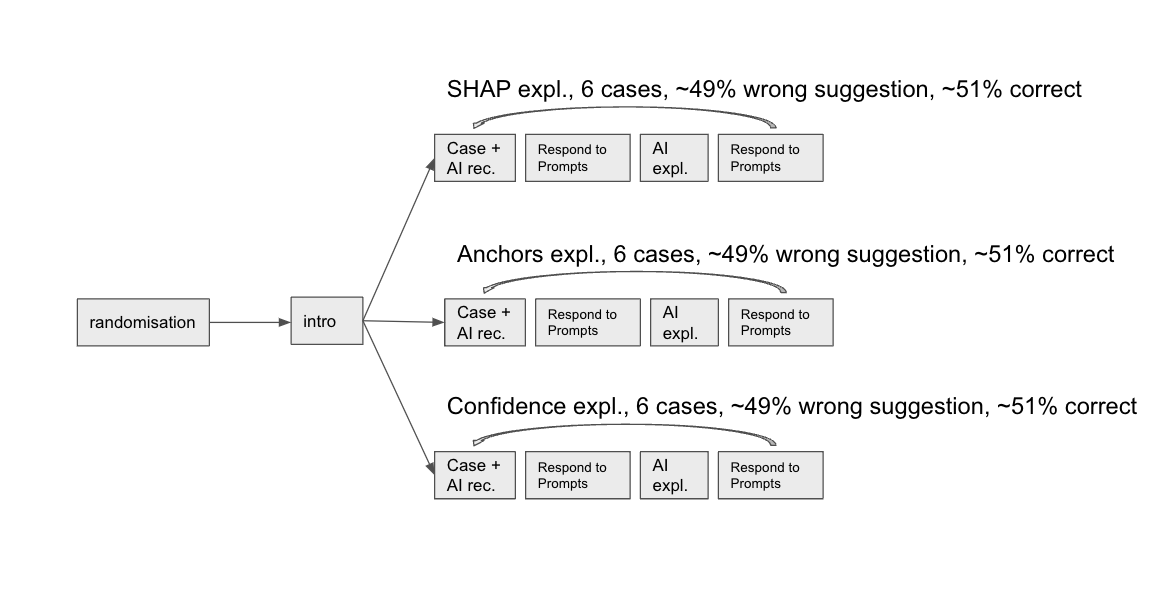
\includegraphics[width=0.8\textwidth]{figures/misleading_explanations/flowchart.png}
    \caption{Study flow}
    \label{fig:flowchart}
\end{figure*}

In both studies, each participant was shown a brief explanation of the task in question and was then asked to complete the 6 cases, with participants given a random mix of correct and incorrect cases. In each case, participants are first shown a table identifying subject of the case and an AI recommendation of what determination they should make. They are then asked to estimate the dependent variable, and rate both their confidence in the estimate and their trust in the AI recommendation on sliding scales (this is discretised to 20 points).

We code the participant's estimate as a binary $estiamte$ variable. The two sliding scale responses are coded as $confidence$ and $trust_{attitude}$ and have values between 1 and 20. As we do this in both the `before-explanation' and `after-explanation' conditions, we collect six responses from each participant in each case:  $estimate^{before}$, $confidence^{before}$, $trust_{attitude}^{before}$, $estimate^{after}$, $confidence^{before}$, and $trust_{attitude}^{after}$.  We additionally have the binary variables $answer$ and $recommendation$ indicating to true value and AI determination of the dependent variable, respectively.

In addition to these, we define $agreement^{before}$ and $agreement^{after}$ to be whether the user's estimate is in agreement with the machine's recommendation. We define $trust_{behaviour}^before$ and $trust_{behaviour}^after$ to be the extent to which the participant's confidence agrees with the machine's recommendation. Finally, in order to reason about the change in a variable due to the explanation, we define `$\Delta$' constructs for all variables with a $before$ and an $after$ case as the after-explanation value minus the before-explanation value.

More detailed definitions of all constructs can be found in Appendix \ref{app:misleadingexplanations}.

\subsection{Demographcs}

We had a total of $192$ participants complete the Salary Estimation study. These were split pseudorandomly into our three explanatory groups. By gender, $115$ were Male, $76$ were Female, and $1$ did not provide gender information. By ethnicity, $137$ were white, $10$ did not provide ethnicity, and the remaining $45$ were split among non-white ethnicities. Our participants were an average of $36.7$ years old, with the oldest being $18$ and the oldest $74$. Each applicant completed an introductory page and six cases. The average completion time for these tasks were $7$ minutes $43$ seconds, the minimum was $2$ minutes $25$, and the maximum was $36$ minutes $46$.

We had a total of $197$ participants complete the Credit Prediction study. These were similarly split into groups. By gender, $106$ were Male, $90$ were Female, and $1$ did not provide gender information. By ethnicity, $143$ were white, $11$ did not provide ethnicity, and the remaining $43$ were split among non-white ethnicities. Our participants were an average of $38.4$ years old, with the oldest being $20$ and the oldest $77$. Each applicant completed an introductory page and six cases. The average completion time for these tasks were $7$ minutes $53$ seconds, the minimum was $2$ minutes $17$, and the maximum was $30$ minutes $13$.

In both tasks, though we originally set $200$ as our target participants, some participants did not complete our task following Prolific Academic's guidelines. Data from these participants was marked incomplete and removed from consideration leaving a total of 192 and 197 participants in each study.

\subsection{SHAP and Confidence Increase Unwarranted Trust}\label{ssec:ttests}
We first test for possible increases in unwarranted trust and find that SHAP and Confidence both increase unwarranted trust on our tasks \cite{natarajan_binns_2022}. That is, when the AI recommendation is incorrect (I.e., when $answer \neq recommendation$), we find that these conditions increase trust. Furthermore, we find this result more strongly for behavioural trust than attitudinal trust in all but one test. Notably, the Anchors condition does not follow this pattern.

Table \ref{tab:delta-trust-t} shows the results of a one-sided t-test comparing $trust^{after}$ to $trust^{before}$ when $answer \neq recommendation$. A positive $t$ statistic indicates $x^{after} > x^{before}$ (I.e., $\Delta x > 0$), and a negative $t$ statistic indicates $x^{after} < x^{before}$, but, as these are one-sided tests, $p$-values will only be meaningful when $t > 0$. We show both types of trust in all three explanatory conditions on both tasks.

\begin{table*}[htbp]
    \caption{One-Sided T-Tests Comparing Trust Before- and After-Explanation}
    \begin{center}
    \begin{tabular}{ccccc}
        \toprule
        Task & Condition & Variable & t Statistic & p Value \\ 
        \midrule
        Salary Estimation & Anchors & $trust_{behaviour}$ & $0.509$ & $0.306$ \\
        & & $trust_{attitude}$ & $0.165$ & $0.434$ \\
        & SHAP & $trust_{behaviour}$ & $\mathbf{3.811}$ & $\mathbf{<0.001}$ \\
        & & $trust_{attitude}$ & $-0.886$ & $0.812$ \\
        & Confidence & $trust_{behaviour}$ & $\mathbf{2.196}$ & $\mathbf{0.015}$ \\
        & & $trust_{attitude}$ & $0.945$ & $0.173$ \\
        \midrule
        Credit Prediction & Anchors & $trust_{behaviour}$ & $1.396$ & $0.082$ \\
        & & $trust_{attitude}$ & $-2.364$ & $0.990$ \\
        & SHAP & $trust_{behaviour}$ & $1.516$ & $0.066$ \\
        & & $trust_{attitude}$ & $\mathbf{2.475}$ & $\mathbf{0.007}$ \\
        & Confidence & $trust_{behaviour}$ & $\mathbf{1.835}$ & $\mathbf{0.034}$ \\
        & & $trust_{attitude}$ & $0.940$ & $0.174$ \\
        \bottomrule
    \end{tabular}
    \label{tab:delta-trust-t}
    \end{center}
\end{table*}

Note that this is only testing for an unwarranted increase in trust, and says nothing about warranted increases or unwarranted decreases. We instrument this test as such because prior work indicates that modern explanation methods are not well-calibrated, leading us to expect such unwarranted increases \cite{miller_explainable_2023}.

\subsection{Different Explanation Styles Have Different Effects on Unwarranted Trust}\label{ssec:anovas}
We next seek to determine whether the change in trust varies between our conditions \cite{natarajan_binns_2022}. We find that such changes in trust do in fact vary between conditions. Further analysis of this variance is found in Subsections \ref{ssec:hsd-salary} and \ref{ssec:hsd-credit}.

Table \ref{tab:delta-trust-anova} contains ANOVA tests examining whether different explanation styles yielded different $\Delta trust$ values when $answer \neq recommendation$. An $F>1$ indicates that different explanation styles (I.e., SHAP, Anchors, and Confidence) have a different impact on the given trust variable, and $p<0.05$ indicates that this difference is statistically significant. However, ANOVA analyses do not indicate \emph{which} styles differ.

\begin{table}[htbp]
    \caption{ANOVAs Comparing Trust Across Explanation Styles}
    \begin{center}
    \begin{tabular}{cccc}
        \toprule
        Task & Variable & F Statistic & p Value \\
        \midrule
        Salary Estimation & $\Delta trust_{behaviour}$ & $\mathbf{3.671}$ & $\mathbf{0.026}$ \\
        & $\Delta trust_{attitude}$ & $0.925$ & $0.397$ \\
        \midrule
        Credit Prediction & $\Delta trust_{behaviour}$ & $0.066$ & $0.936$ \\
        & $\Delta trust_{attitude}$ & $\mathbf{6.213}$ & $\mathbf{0.002}$ \\
        \bottomrule
    \end{tabular}
    \label{tab:delta-trust-anova}
    \end{center}
\end{table}

In the Salary Estimation task, we find no significant results for our ANOVA $trust_{attitude}$, but do find significant results for $trust_{behaviour}$. However, in the Credit Prediction task, we find significant results for our ANOVA $trust_{attitude}$, but none for $trust_{behaviour}$. That is, in the Salary Estiamtion task, different explanations styles have a different impact on behavioural trust, and in the Credit Prediction task, different explanations styles have a different impact on attitudinal trust. We examine these two findings in Subsections \ref{ssec:hsd-salary} and \ref{ssec:hsd-credit}, respectively.

\subsubsection{SHAP Increases Behavioural Trust More than Anchors in the Salary Estimation Task}\label{ssec:hsd-salary}
We would expect that, because we found that $\Delta trust_{behaviour} > 0$ in both the SHAP and Confidence cases of the Salary Estimation Task (and in the Anchors case we did not), the means of the former two should be significantly greater than the latter. However, while we find that SHAP increases behavioural trust more than Anchors, we find no significant results relating to the Confidence condition.

Following our preregistered protocol for significant ANOVA results, we turn to Tukey's HSD as a post-hoc test \cite{natarajan_binns_2022}. Table \ref{tab:delta-trust-hsd} shows the results of this test. Note that this is again restricted to when $answer \neq recommendation$.

\begin{table}[htbp]
    \caption{Tukey's HSD Test Comparing Change in Behavioural Trust Across Explanations in Salary Estimation}
    \begin{center}
    \begin{tabular}{ccccc}
        \toprule
        Condition A & Condition B & Variable & Test Statistic & p Value \\
        \midrule
        SHAP & Anchors & $\Delta trust_{behaviour}$ & $\mathbf{2.310}$ & $\mathbf{0.022}$ \\
        Confidence & Anchors & $\Delta trust_{behaviour}$ & $0.855$ & $0.599$ \\
        SHAP & Confidence & $\Delta trust_{behaviour}$ & $1.455$ & $0.198$ \\
        \bottomrule
    \end{tabular}
    \label{tab:delta-trust-hsd}
    \end{center}
\end{table}

Table \ref{tab:delta-trust-hsd} demonstrates a significant difference in the mean of $\Delta trust_{behaviour}$ only between the SHAP and Anchors conditions when $answer \neq recommendation$. This indicates that, beyond increasing behavioural trust in incorrect AI outputs, SHAP increases behavioural trust in incorrect AI outputs \emph{more} than Anchors.

\subsubsection{SHAP and Confidence Increase Unwarranted Attitudinal Trust More than Anchors in the Credit Prediction Task}\label{ssec:hsd-credit}
We found a large negative $t$ value for $\Delta trust_{attitude}$ in the Anchors case in the Credit Prediction portion of Table \ref{tab:delta-trust-t} -- an effect that is not significant due to the one-sidedness of our tests. However, as we found only positive $t$ values for $\Delta trust_{attitude}$ in the SHAP and Confidence cases, we expect that Anchors has a negative effect on $\Delta trust_{attitude}$ relative to SHAP and Confidence. Table \ref{tab:delta-trust-anova} confirms this expectation: SHAP and Confidence both have a more positive effect on attitudinal trust than Anchors in the Credit Prediction task.

Table \ref{tab:delta-trust-anova} again follows our preregistered protocol for significant ANOVA results with a Tukey's Honestly Significant Difference (HSD) test \cite{natarajan_binns_2022}. This is again restricted to when $answer \neq recommendation$.

\begin{table}[htbp]
    \caption{Tukey's HSD Test Comparing Change in Attitudinal Trust Across Explanations in Credit Prediction}
    \begin{center}
    \begin{tabular}{ccccc}
        \toprule
        Condition A & Condition B & Variable & Test Statistic & p Value \\
        \midrule
        SHAP & Anchors & $\Delta trust_{attitude}$ & $\mathbf{1.213}$ & $\mathbf{<0.001}$ \\
        Confidence & Anchors & $\Delta trust_{attitude}$ & $\mathbf{1.030}$ & $\mathbf{<0.001}$ \\
        SHAP & Confidence & $\Delta trust_{attitude}$ & $0.183$ & $0.708$ \\
        \bottomrule
    \end{tabular}
    \label{tab:delta-trust-hsd-2}
    \end{center}
\end{table}

Table \ref{tab:delta-trust-hsd-2} shows a significant difference in the mean of $\Delta trust_{behaviour}$ between the Anchors condition and both other conditions, but no significant difference between SHAP and Confidence. This indicates that SHAP and Confidence increase unwarranted attitudinal trust relative to Anchors (although Anchors appears to actually \emph{reduce} unwarranted attitudinal trust).

Note that this does not prove that Anchors reduces attitudinal trust relative to no explanation. For this analysis, we will need another t-test. As we did not preregister this test, analysis of this phenomenon is included in exploratory analysis in Subsection \ref{ssec:anchors-decrease} \cite{natarajan_binns_2022}.

\subsection{Anchors Decrease Attitudinal Trust in a Machine}\label{ssec:anchors-decrease}
We noted already that SHAP and Confidence appear to increase trust in cases where the machine is incorrect. However, we noticed no such result for Anchors. Instead, we found that Anchors appeared to decrease end-user trust in incorrect machine outputs (I.e., when $answer \neq recommendation$). The two-sided t-test in table \ref{tab:delta-trust-t-2} confirms this.\footnote{This analysis was not preregistered.}

\begin{table*}[htbp]
    \caption{Two-Sided T-Tests Comparing Trust Before- and After-Explanation}
    \begin{center}
    \begin{tabular}{ccccc}
        \toprule
        Task & Condition & Variable & t Statistic & p Value \\ 
        \midrule
        Salary Estimation & Anchors & $trust_{behaviour}$ & $0.509$ & $0.611$ \\
        & & $trust_{attitude}$ & $0.165$ & $0.869$ \\
        \midrule
        Credit Prediction & Anchors & $trust_{behaviour}$ & $1.396$ & $0.164$ \\
        & & $trust_{attitude}$ & $\mathbf{-2.364}$ & $\mathbf{0.019}$ \\
        \bottomrule
    \end{tabular}
    \label{tab:delta-trust-t-2}
    \end{center}
\end{table*}

Table \ref{tab:delta-trust-t-2} shows that, on the two-sided t-test, we \textit{do} find that the provision of Anchors explanations decreases participant attitudinal trust in incorrect machine recommendations, at least in the Credit Prediction task. However, we do not see a similar effect on behavioural trust, and this effect is limited to only one task. 

\subsection{Behavioural and Attitudinal Trust are Highly Correlated}\label{ssec:trust-corr}
Given that many patterns observed for $trust_{behaviour}$ do not hold for $trust_{attitude}$, we might expect these variables to correlate only minimally. However, while they are mathematically distinct constructs, they are both intended to measure the same underlying phenomenon. Table \ref{tab:trust-correlation} demonstrates a high correlation between these two measurements of trust across all cases.\footnote{Though previous analyses considered only incorrect recommendations, this analysis relates \textit{all} trust, not just unwarranted trust, so we consider all cases, regardless of whether or not $answer == recommendation$.}\footnote{This analysis was only partially preregistered; we did not register this analysis in the Salary Estimation task, but we did in the Credit Prediction task \cite{natarajan_binns_2022}.}

Table \ref{tab:trust-correlation} shows a Pearson's correlation analysis across all explanatory conditions in both the before- and after- cases. We also perform this analysis on $\Delta trust_{attitude}$ and $\Delta trust_{behaviour}$.

\begin{table*}[htbp]
    \caption{Pearson's Correlation Between Attitudinal and Behavioural Trust}
    \begin{center}
    \begin{tabular}{ccccc}
        \toprule
        Task & Variable A & Variable B & Rho & p Value \\
        \midrule
        Salary Estimation & $trust_{attitude}$ & $trust_{behaviour}$ & $\mathbf{0.630}$ & $\mathbf{<0.001}$ \\
        & $\Delta trust_{attitude}$ & $\Delta trust_{behaviour}$ & $\mathbf{0.265}$ & $\mathbf{<0.001}$ \\
        \midrule
        Credit Prediction & $trust_{attitude}$ & $trust_{behaviour}$ & $\mathbf{0.612}$ & $\mathbf{<0.001}$ \\
        & $\Delta trust_{attitude}$ & $\Delta trust_{behaviour}$ & $\mathbf{0.179}$ & $\mathbf{<0.001}$ \\
        \bottomrule
    \end{tabular}
    \label{tab:trust-correlation}
    \end{center}
\end{table*}

Table \ref{tab:trust-correlation} indicates that both trust variables are highly correlated across both of our tasks. Furthermore, though the correlation between the $\Delta trust$ is more modest, it is still statistically significant.

\subsection{Anchors and SHAP Increase Participant Confidence in their Prediction}

Noting that behavioural trust is constructed from $confidence$ values, we ask: ``does providing an Anchors explanations increase participant confidence in their own decisions when the AI recommendation is incorrect?'' Table \ref{tab:delta-trust-t} supplies evidence indicating that Anchors (and SHAP) explanations increase participant confidence in their own estimations when $answer \neq recommendation$. This result agrees with \textcite{wan_explainabilitys_2022} and \textcite{bansal_does_2021}, suggesting these explanation types yield a blanket increase in participant self-confidence.\footnote{This analysis was not preregistered.}

Table \ref{tab:delta-confidence-t} contains a t-test comparing $confidence$ in all three explanatory conditions. \footnote{Note for clarity that $confidence$ is the variable indicating participant confidence in their own decisions, and `Confidence' is the condition in which the machine's explanation consists of its own confidence in its suggestion.}

\begin{table}[htbp]
    \caption{One-Sided T-Tests Comparing $confidence$ Before- and After-Explanation}
    \begin{center}
    \begin{tabular}{ccccc}
        \toprule
        Task & Condition & Variable & t Statistic & p Value \\
        \midrule
        Salary Estimation & Anchors & $confidence$ & $\mathbf{2.171}$ & $\mathbf{0.016}$ \\
        & SHAP & $confidence$ & $\mathbf{1.694}$ & $\mathbf{0.046}$ \\
        & Confidence & $confidence$ & $1.047$ & $0.296$ \\
        \midrule
        Credit Prediction & Anchors & $confidence$ & $\mathbf{1.742}$ & $\mathbf{0.042}$ \\
        & SHAP & $confidence$ & $\mathbf{3.473}$ & $\mathbf{<0.001}$ \\
        & Confidence & $confidence$ & $0.752$ & $0.226$ \\
        \bottomrule
    \end{tabular}
    \label{tab:delta-confidence-t}
    \end{center}
\end{table}

Table \ref{tab:delta-trust-t} demonstrates that, while Confidence shows no significant effects on either task, participants shown an Anchors or SHAP explanation grow significantly more confident in their prediction, indicating that providing an Anchors or SHAP explanation serves to increase a participant's confidence in their \emph{own estimate}.

\subsection{Explanations Impact Trust Differently When the Machine is Correct}
Note that properly calibrated trust would involve both distrusting the machine when it is wrong and trusting it when it is right. To assess the latter, we give a brief evaluation of what happens in the cases where the AI is correct, I.e. where $answer == recommendation$. Table \ref{tab:delta-trust-t-positives} contains the results of these analyses.\footnote{These analyses were not preregistered.}

\begin{table*}[htbp]
    \caption{Two-Sided T-Tests Comparing Trust Before- and After-Explanation when $answer == recommendation$}
    \begin{center}
    \begin{tabular}{ccccc}
        \toprule
        Task & Condition & Variable & F Statistic & p Value \\ 
        \midrule
        Salary Estimation & Anchors & $trust_{behaviour}$ & $0.502$ & $0.616$ \\
        & & $trust_{attitude}$ & $\mathbf{-2.337}$ & $\mathbf{0.020}$ \\
        & SHAP & $trust_{behaviour}$ & $0.295$ & $0.768$ \\
        & & $trust_{attitude}$ & $-1.385$ & $0.168$ \\
        & Confidence & $trust_{behaviour}$ & $\mathbf{2.410}$ & $\mathbf{0.017}$ \\
        & & $trust_{attitude}$ & $\mathbf{3.254}$ & $\mathbf{0.001}$ \\
        \midrule
        Credit Prediction & Anchors & $trust_{behaviour}$ & $\mathbf{3.013}$ & $\mathbf{0.003}$ \\
        & & $trust_{attitude}$ & $\mathbf{-2.487}$ & $\mathbf{0.014}$ \\
        & SHAP & $trust_{behaviour}$ & $0.207$ & $0.836$ \\
        & & $trust_{attitude}$ & $\mathbf{3.538}$ & $\mathbf{0.001}$ \\
        & Confidence & $trust_{behaviour}$ & $\mathbf{2.863}$ & $\mathbf{0.005}$ \\
        & & $trust_{attitude}$ & $\mathbf{2.461}$ & $\mathbf{0.015}$ \\
        \bottomrule
    \end{tabular}
    \label{tab:delta-trust-t-positives}
    \end{center}
\end{table*}

\subsubsection{Confidence Explanations Increase Warranted Trust}
Positive $\Delta trust$ values in all cases in table \ref{tab:delta-trust-t-positives} demonstrate that Confidence explanations increased both measured types of user trust in the AI output when the model is correct across both tasks.

\subsubsection{Anchors Explanations Decrease Warranted Attitudinal Trust}
Table \ref{tab:delta-trust-t-positives} also demonstrates that providing Anchors explanations yields a \emph{decrease} in $trust_{attitude}$. This, alongside the finding from Subsection \ref{ssec:anchors-decrease}, indicates that Anchors explanations have a negative impact on $trust_{attitude}$, regardless of model correctness.

\subsubsection{SHAP Explanations Increase Warranted Attitudinal Trust in the Credit Prediction Task}
SHAP explanations increase Warranted attitudinal trust in the Credit Prediction Task as shown in table \ref{tab:delta-trust-t-positives}. However, the effect is not mirrored in tests of $trust_{behaviour}$ or on the Salary Estimation Task.

\subsection{Limitations}

\subsubsection{Generalisation and External Validity}
The external validity of our results may be challenged due to our use of artificial tasks and benchmark datasets. Indeed, field studies with decision-makers in real deployments would be needed to yield results that apply uncontroversially in a given domain. Along a similar vein, one might contend that the use of only two tasks is insufficient to generalise our results to other domains. One might also challenge external validity of our results due to our limited selection of only three explanatory conditions (only two of which are commonly used xAI methods).

We choose two similar datasets in a narrow domain (human-in-the-loop binary classification tasks with definite but non-obvious ground truth) as we do not wish to confuse our primary research questions with questions surrounding generalisation. Similarly, we contend research on further tasks is extraneous to the primary questions. More information on our specific selection of cases can be found in Appendix \ref{app:misleadingexplanations}.

We choose SHAP and Anchors as popular candidate explanations from different styles, as we wish to demonstrate conditions under which unwarranted trust may and may not arise. We choose Confidence as a third condition as this condition acts as a sort of baseline. More information on our choice of explanation algorithms can be found in Appendix \ref{app:misleadingexplanations}.

That said, insofar as performance on benchmark datasets can be expected to generalise, we believe our findings will extend to predictive tasks whose answers are difficult enough to both human and AI systems and where performance is distributed differently between them. We do not expect our findings to generalise to tasks where the answers are either immediately evident to the user (such as predicting whether a given image contains a cat) or so difficult as to be impossible to the naked eye (such as gene function prediction). And while we do expect our findings to generalise beyond tabulated binary classification tasks, said generalisation does not impact the primary significance of these findings: xAI developers, evaluators, and implementers alike should concern themselves with the possibility of unwarranted trust.

\subsubsection{Effect on Overall Task Performance}

We have focused exclusively on the phenomenon of misplaced trust when the AI output is incorrect. However, while problematic, this has to be weighed against the effect an xAI method has on overall task performance. It might be remarked that, even if SHAP explanations increased misplaced trust, if they increased performance on the task overall, that would still be desirable. Indeed, relative to no explanation at all, SHAP may be beneficial simply because of its effect of increasing user trust overall. (The effect of an overall increase in trust in AI outputs will depend on the relative accuracies of the AI and the human.)

However, we do not contend that the unwarranted trust issue renders SHAP explanations useless. We instead contend that they may lead to dangerous abuse. When implementing xAI algorithms in human-in-the-loop tasks, implementers should consider the possible harms of this potential for abuse, especially when these tasks have definite but unobvious ground truth. Furthermore, those developing xAI applications for use in these contexts should strive to develop explanation methods that appropriately calibrate trust in addition to increasing overall task performance.

\subsection{Discussion}
In this chapter, we investigate the extent to which three different AI explanation methods can create unwarranted trust in their underlying AI systems on a specific set of tasks. Specifically, we look at whether any of our Anchors, SHAP, or Confidence explanatory conditions increase trust in a model when that model is wrong. We restrict our analysis specifically to the subset of tasks human-in-the-loop where the ground truth of the prediction is neither subjective nor immediately evident to the human. We perform analyses on two tabular binary prediction tasks that satisfy this condition: Salary Estimation and Credit Prediction.

We conclude here that SHAP and Confidence explanations are liable to induce unwarranted trust under these circumstances, but we find no evidence of the same for Anchors. This demonstrates that, in these cases, neither SHAP nor Confidence serve to correctly calibrate trust in AI outputs. Rather, they blindly increase trust in these outputs, encouraging users to incorrectly agree with the AI explained. Furthermore, we find that, while Anchors may not induce unwarranted trust, it instead fosters blanket distrust for the AI and increased confidence in user decision-making. As such, the effect of Anchors explanations on trust calibration may not be positive overall; it is dependent on the distribution of correct vs. incorrect disagreements between user and AI. (Indeed, for certain distributions of correct vs. incorrect disagreements, all three explanation styles may have a negative overall effect on trust calibration.) These findings suggest that, at least under the conditions outlined, xAI may be at best useless and at worst actively harmful in its effects on human trust calibration. 

Though trust is often a component of both design and evaluation, \emph{trustworthiness} is often overlooked \cite{jacovi_formalizing_2021,lundberg_unified_2017,ribeiro_why_2016,jacobs_how_2021}. It is often assumed that these explanations draw directly from model outputs, and are therefore akin to oracles that grant a general understanding of the system. In \textcite{natarajan_trust_2023}, we argue for a paradigm shift against this use of explainable AI systems, and instead argue that systems should be developed, evaluated, and used for specific purposes. We agree with this sentiment. In fact, we contend it is not itself problematic that user trust in AI systems might increase as a result of xAI. But it is problematic that user trust in wrong decisions made by AI systems may increase in response to the use of a maximally trust-inducing explanation method. Particularly in human-in-the-loop tasks with definite but unclear ground truth, trust should not be considered the \emph{raison d'etre} of xAI. More heed should be instead paid to \emph{calibrating} trust in AI systems and to ensuring that explanations are sufficiently well-calibrated for the use cases they are considered for.

\section{Conclusion}
% Clearly, post-hoc and intrinsically interpretable are very different. We clearly need to study them separately. That's what the next two chapters do